% Short Sectioned Assignment
% LaTeX Template
% Version 1.0 (5/5/12)
%
% This template has been downloaded from:
% http://www.LaTeXTemplates.com
%
% Original author:
% Frits Wenneker (http://www.howtotex.com)
%
% License:
% CC BY-NC-SA 3.0 (http://creativecommons.org/licenses/by-nc-sa/3.0/)
%
%%%%%%%%%%%%%%%%%%%%%%%%%%%%%%%%%%%%%%%%%

%----------------------------------------------------------------------------------------
%	PACKAGES AND OTHER DOCUMENT CONFIGURATIONS
%----------------------------------------------------------------------------------------

\documentclass[paper=a4, fontsize=11pt]{scrartcl} % A4 paper and 11pt font size

\usepackage[T1]{fontenc} % Use 8-bit encoding that has 256 glyphs
\usepackage[english]{babel} % English language/hyphenation
\usepackage{amsmath,amsfonts,amsthm} % Math packages


\usepackage{graphicx}
\usepackage{subfig}
\usepackage{amssymb}
\usepackage{hyperref}
\usepackage{float}

\usepackage{multicol}
\usepackage{mdwlist}
\usepackage{fancyhdr} % Custom headers and footers
\pagestyle{fancyplain} % Makes all pages in the document conform to the custom headers and footers
\fancyhead{} % No page header - if you want one, create it in the same way as the footers below
\fancyfoot[L]{} % Empty left footer
\fancyfoot[C]{} % Empty center footer
\fancyfoot[R]{\thepage} % Page numbering for right footer
\renewcommand{\headrulewidth}{0pt} % Remove header underlines
\renewcommand{\footrulewidth}{0pt} % Remove footer underlines
\setlength{\headheight}{6pt} % Customize the height of the header

\numberwithin{equation}{section} % Number equations within sections (i.e. 1.1, 1.2, 2.1, 2.2 instead of 1, 2, 3, 4)
\numberwithin{figure}{section} % Number figures within sections (i.e. 1.1, 1.2, 2.1, 2.2 instead of 1, 2, 3, 4)
\numberwithin{table}{section} % Number tables within sections (i.e. 1.1, 1.2, 2.1, 2.2 instead of 1, 2, 3, 4)

\setlength\parindent{0pt} % Removes all indentation from paragraphs - comment this line for an assignment with lots of text

%----------------------------------------------------------------------------------------
%	TITLE SECTION
%----------------------------------------------------------------------------------------

\newcommand{\horrule}[1]{\rule{\linewidth}{#1}} % Create horizontal rule command with 1 argument of height

\title{	
\normalfont \normalsize 
\textsc{UC Berkeley, Computer Science} \\ [25pt] % Your university, school and/or department name(s)
\horrule{0.5pt} \\[0.4cm] % Thin top horizontal rule
\huge Gender Classification of Handwritten Text \\ % The assignment title
\horrule{2pt} \\[0.5cm] % Thick bottom horizontal rule
}

\author{Peter Cheng, Jeff Tsui, Alice Wang} % Your name

\date{\normalsize\today} % Today's date or a custom date

\begin{document}

\maketitle % Print the title

\section{Introduction}
For our project we designed and tested an off-line classifier for
gender prediction, using handwritten text. The inspiration for this
project came from a Kaggle machine learning competition
\cite{kaggle}. Kaggle provides sample training data, in the form of
high-resolution (300 dpi) jpg images. Each image corresponds to a
writing sample, and there are 4 writing samples for each of 475
writers. The 4 samples correspond to:

\begin{enumerate}
\item Arabic text, different text for each writer
\item Arabic text, same text for each writer
\item English text, different text for each writer
\item English text, same text for each writer
\end{enumerate}

Section \ref{sec:background} provides some details that lead to
preprocessing and feature extraction. Section \ref{sec:pands} details
the preprocessing tasks we performed on the Kaggle jpg images
provided. Section \ref{sec:feature} describes in detail the
methodology behind feature extraction of the processed images. Section
\ref{sec:results} demonstrates the performance of our extracted features
using various canonical classifiers.

\section{Background}
\label{sec:background}
For this particular contest, Kaggle provided 700+ extracted features
for each writing sample. Upon examining relevant literature, we
concluded that generating relevant features is as important, if not
more so than honing the optimal classification model. We diverged our
project to focus on our own feature extraction. In order to do so on
the highly unconstrained Kaggle dataset, we will perform a number of
preprocessing steps.

The data we used consists of only the fourth sample for each writer,
which is the same English text written by each writer. Since the data
supplied is for a competition, the test data did not have gender
labels. We decided to limit our dataset to the labeled training data,
where label = 1 for male and label = 0 for female. Of these 282
writing samples, we reserved
25\% to be our own testing set. An example of a sample document image is shown in Figure \ref{fig:docImage}.

\begin{figure}
\centering \fbox{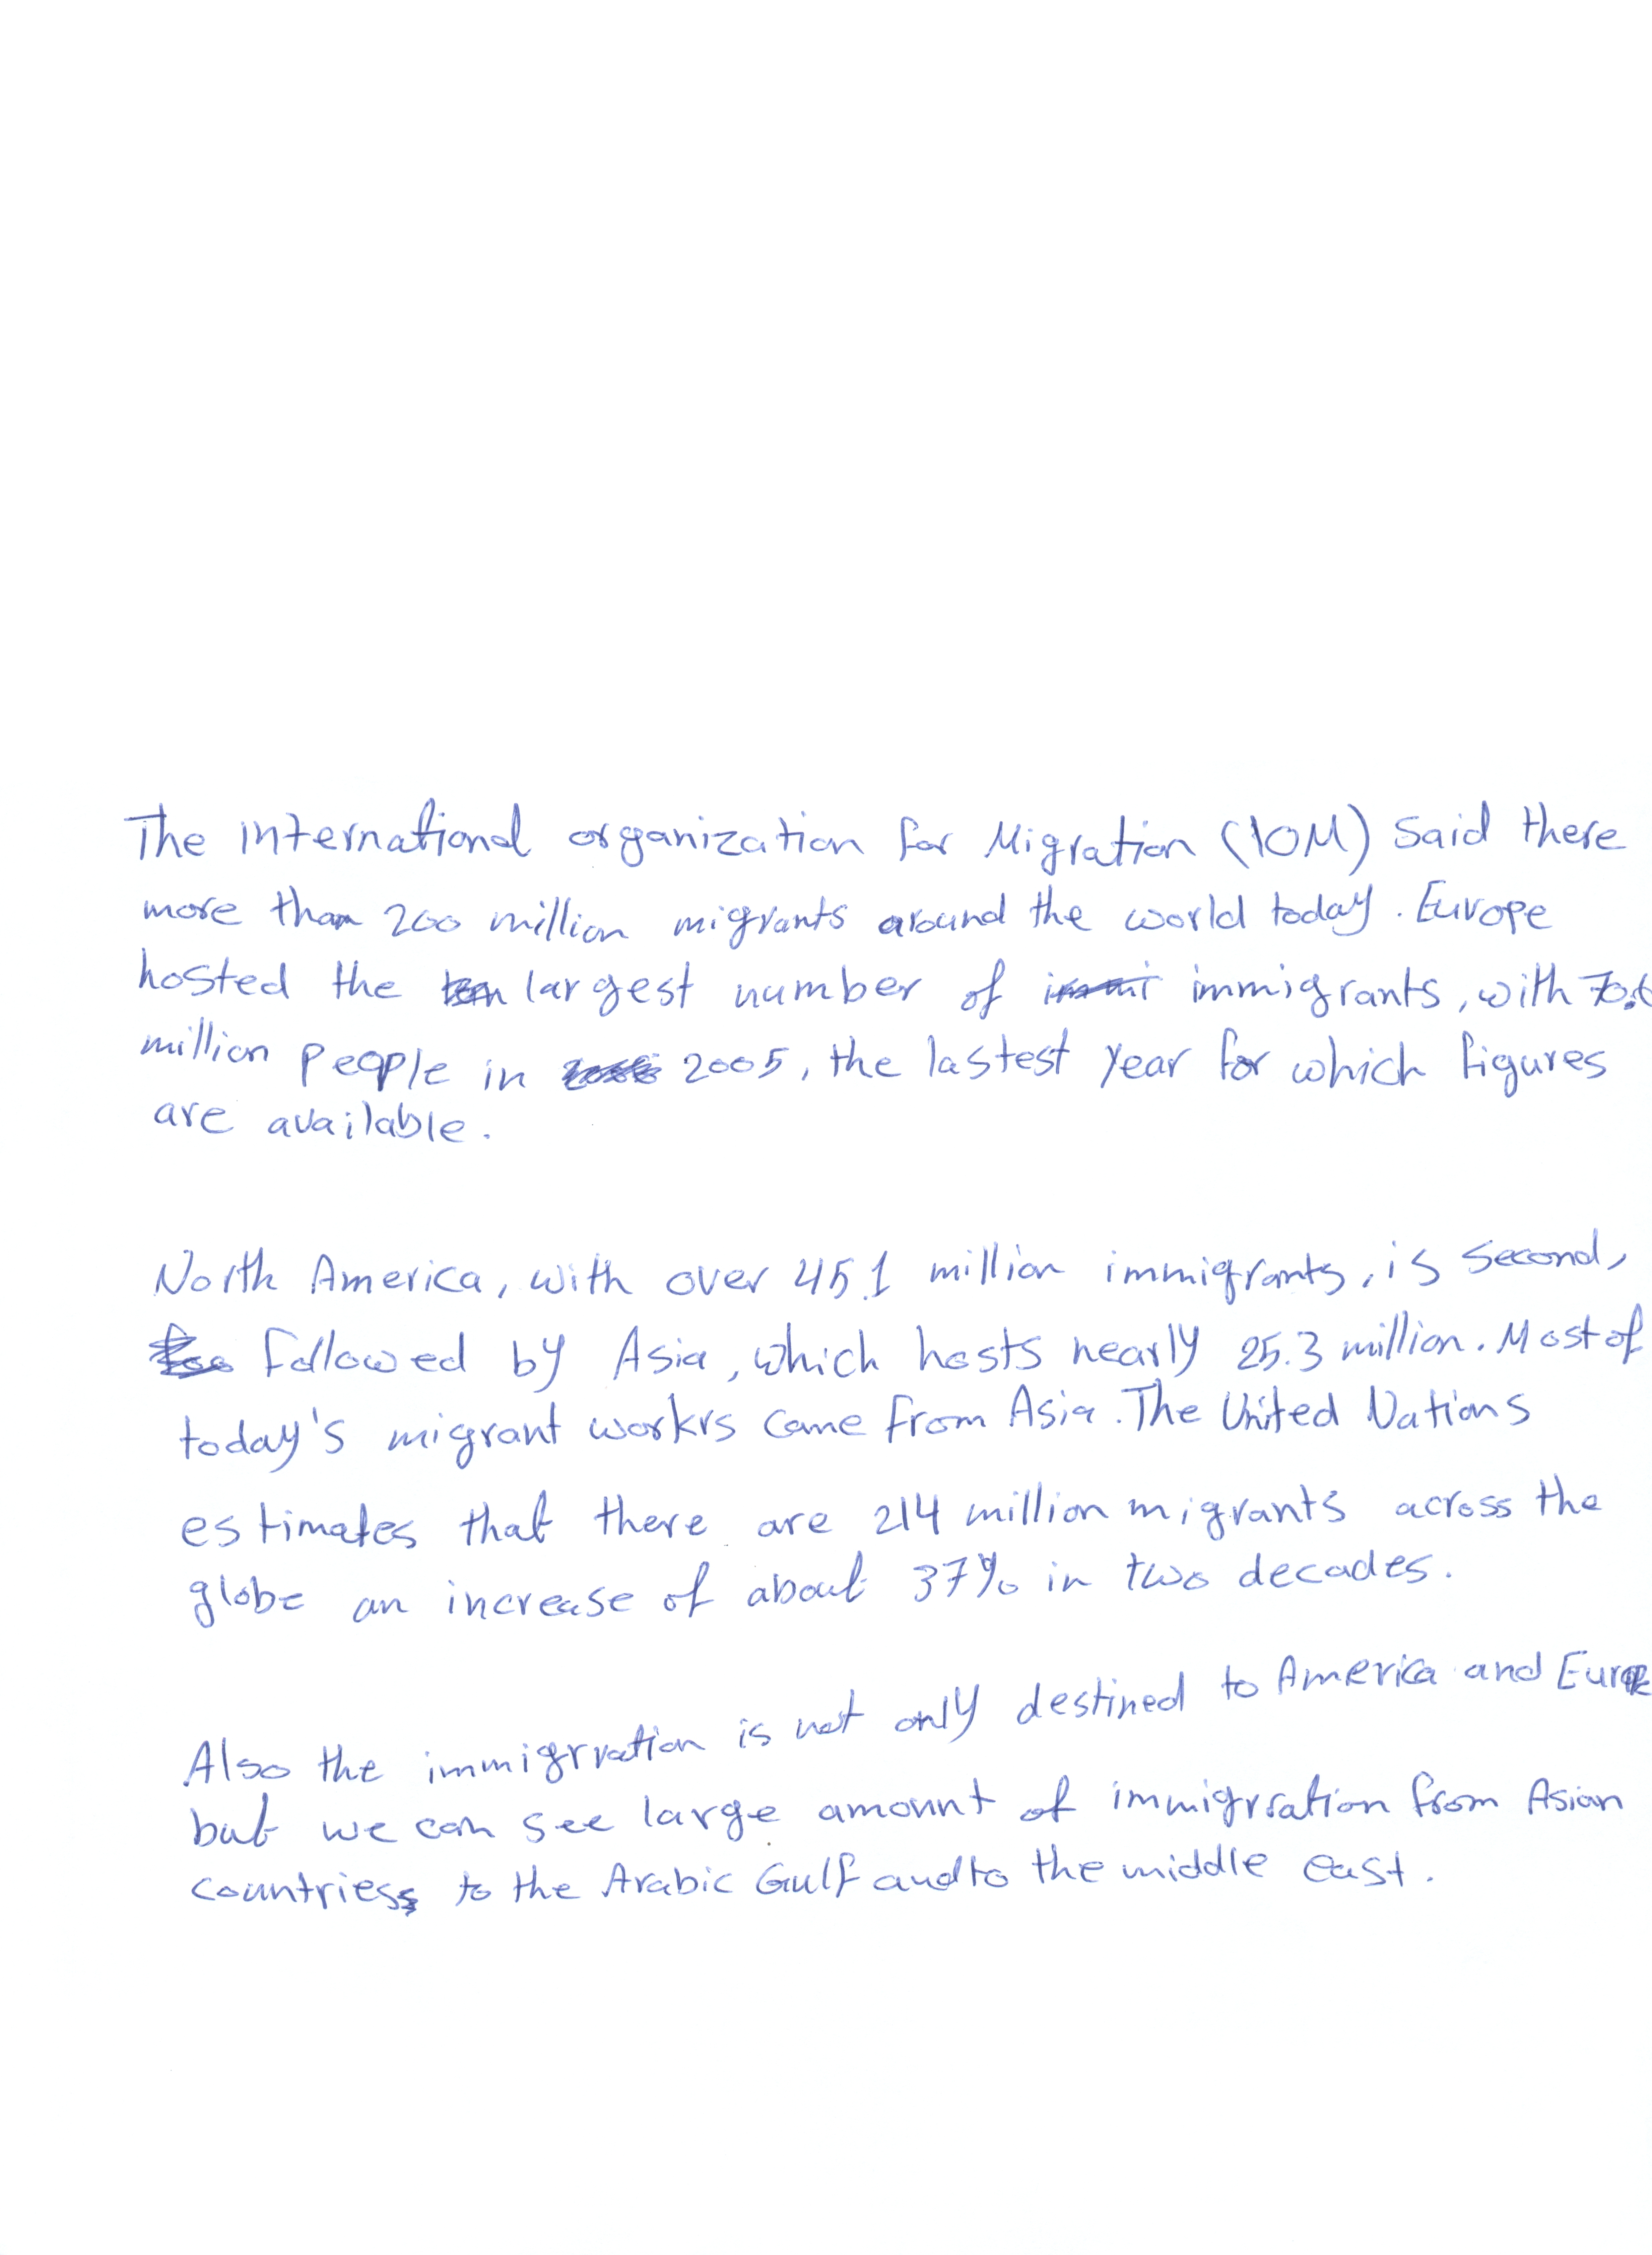
\includegraphics[width=4in, height=5in]{docimage.jpg}}
\caption{A sample input document image}
\label{fig:docImage}
\end{figure}

We started with trying to classify our dataset with each character's
appearance via Optical Character Recognition, and quickly concluded
that it introduced more error and uncertainty than necessary. Instead,
we perform a number of preprocessing and segmentation steps described
in the next section. In this paper we refer to document image and word
image, or line image, where each is an image containing a single
document, word, or line respectively separately. Using the processed
images, we generate a set of 56 features for each line. Then we
calculate error rates from building several classification models, and
summarize the results below.

\section{Preprocessing and Segmentation}
\label{sec:pands}
Typically, when performing handwriting classification and feature
extraction, binary images with a number of constraints are
assumed. Typical constraints seen in previous work include having
images in black and white, text all equally scaled among different
writers, and lines written at consistent angles
\cite{Preprocessing}. Furthermore, many feature extraction approaches
are tuned to work on images of individual characters, words, or lines,
instead of an entire document altogether. As a result, before
extracting features, we perform a series of preprocessing steps, to
normalize each document image \footnote{in this paper we refer to
document image, word image, or line image, where each is an image
containing a single document, word, or line respectively.}, followed
by segmentation procedures to segment out lines and words.

\subsection{Preprocessing}
The first step in preprocessing is to translate each input color image
into a binary black and white image. To accomplish this, an intensity
threshold is calculated, such that pixels with intensity above that
value are set to 1, while the rest are set to 0. This intensity
threshold is calculated using Matlab's ``graythresh'' function, which
performs Otsu's method for binary thresholding
\cite{ThresholdSelection}. Following this binarization, we then trim
off the margins of each image, as writing samples are centered around
different locations on the page. This is done simply by retaining the
image within the minimum axis-aligned bounding box containing all text
in the image.

\subsection{Segmentation}
While features that are calculated on handwriting samples could
theoretically be extracted from entire document images all at once,
many of the features we use are specific to words or lines, so it
makes sense to first break down the input space into line images and
word images, so as to potentially reduce error when extracting these
features.

\subsubsection{Line Segmentation}

\begin{figure}
  \centering \includegraphics[width=4in, height=4in]{linesdetected.jpg}
  \caption{Line segments detected on a document image roughly
    correspond to lines of text}
\label{fig:houghLineDetect}
\end{figure}

To perform line segmentation, the Hough-transform-based algorithm
proposed by Louloudis, G., et al, \cite{BlockBased} is loosely
followed. First, we use Matlab's probabilistic Hough line segment
detector (HoughlinesP) implementation to detect lines on the document
images, preprocessed after the previous section. We restrict Hough
peak detection to only occur in the angle domain such that detected
lines deviate at most 5 degrees from horizontal. We bin angles at a
resolution of 1 degree, and the rho parameter at a resolution of 1
pixel. The parameters for minimum line length and maximum gap within a
line are more important, and are set to be 75\% of the image's width
and 10\% of the image's width. An example of such detected lines is
shown in Figure \ref{fig:houghLineDetect}. Each detected line is then
drawn onto the word image, such that pixel values corresponding to the
line are set to 1. Now, connected components are detected on the image
with lines added, and if accurate lines were detected, each character
and word in a line of text should all be in one contiguous connected
component, held together by the lines drawn over them. Connected
components with fewer than 10000 pixels are filtered out, as are those
with a width less than 8 times the height, as the former case
corresponds to punctuation or characters that were not properly
grouped, while the latter case corresponds to cases where multiple
lines of text were detected together. Each connected component,
(without the detected lines), is now output at as a separate line
image without the lines on top. 

In some cases, our line segmentation technique was unable to correctly separate adjacent lines, where we are unable to correctly separate the two lines. This is seen in Figure \ref{fig:linefail}, where the lines are written very closely together and there is a slight angle to each line, where the first line dips in the center slightly and the second line slants downwards. These factors make it difficult to perform line segmentation.

\begin{figure}
\centering \includegraphics{linefail.png}
\caption{In this case, line segmentation failed to perform properly because two lines were very close together and a single detected line segment spanned both lines.}
\label{fig:linefail}
\end{figure}

\subsubsection{Word Segmentation}
The word segmentation procedure we use is similar to the line
segmentation method described in the previous section. Essentially,
smaller lines are detected within each line image, such that
individual words become the connected components. For this application
we use the same angle and offset thresholds and resolutions as before,
but set the minimum line length to be 2\% of the line image's width,
while the maximum gap in a line is 1.5\% of the line image's
width. After after filtering out connected components with fewer than
500 pixels, we can then extract word images via the connected
components.

It is useful to have words that are rotated such that their baseline
is horizontal during feature extraction. Caesar, T., et al [2] cite a
number of approaches to accomplish this, but we took a fairly simple
approach. For each word, we computed its (rotated) bounding box, and
rotated the image such that the bounding box is axis-aligned. As seen
in Figure \ref{fig:wordfail}, this worked well for a high percentage
of words but did not in certain cases. The writer used cursive writing
with little spacing between consecutive words, which resulted in the
three words “there”, “are”, and “21” being are segmented as one word.

\begin{figure}
  \centering \includegraphics{wordfail.png}
  \caption{A case where word segmentation does not perform properly,
    as adjacent words are connected.}
  \label{fig:wordfail}
\end{figure}


\section{Feature Extraction}
\label{sec:feature}
In this section, we describe the features recovered from line images
and word images, after preprocessing and segmentation, as described in
the previous two sections. A listing of each feature is shown in
Figure \ref{fig:featureList}

\begin{figure}
  \begin{multicols}{3}
    \begin{enumerate*}
    \item Upper baseline to top line distance
    \item Lower baseline to upper baseline distance
    \item Bottom line to lower baseline distance
    \item 1 / 2
    \item 1 / 3
    \item 2 / 3
    \item Median of the gap lengths
    \item 2 / 7
    \item Average slant angle
    \item Std dev of slant angles
    \item Line angle
    \item Slant of lower contour
    \item Mean squared error of lower contour
    \item Freq of local max for lower contour
    \item Freq of local min for lower contour
    \item Avg left slope of local max for lower contour
    \item Avg right slope of local max for lower contour
    \item Avg left slope of local min for lower contour
    \item Avg right slope of local min for lower contour
    \item 12 for upper contour
    \item 13 for upper contour
    \item 14 for upper contour
    \item 15 for upper contour
    \item 16 for upper contour
    \item 17 for upper contour
    \item 18 for upper contour
    \item 19 for upper contour
    \item Avg width of connected components
    \item Avg height of connected components
    \item Std dev of width of ccs
    \item Std dev of height of ccs
    \item Avg dist between adjacent ccs
    \item Std dev of dist between adjacent ccs
    \item Avg area of enclosed regions
    \item Avg length of major axis of ers
    \item Avg length of minor axis of ers
    \item Avg orientation of ers
    \item Avg eccentricity of ers
    \item Avg equiv diameter squared of ers
    \item Avg extent of ers
    \item Avg perimeter of ers
    \item Avg form factor of ers
    \item Avg roundness of ers
    \item Std dev of 34
    \item Std dev of 35
    \item Std dev of 36
    \item Std dev of 37
    \item Std dev of 38
    \item Std dev of 39
    \item Std dev of 40
    \item Std dev of 41
    \item Std dev of 42
    \item std dev of 43
    \item Fractal dimension slope 1
    \item Fractal dimension slope 2
    \item Fractal dimension slope 3
    \end{enumerate*}
  \end{multicols}
  \caption{The features we extracted from each input document image}
  \label{fig:featureList}
\end{figure}

\subsection{Word Features}
The first group of features are generated based on word images,
referencing the work of Marti, U.-V., et al \cite{WriterID} where a
feature vector is extracted from each word. These feature vectors are
averaged by line to combine them with line-specific feature
vectors. The word features include the width, slant, and height of the
three main writing zones.

\subsubsection{Word Height}
The three writing zones are separated by the upper and lower
baselines. The upper and lower baselines are defined via analysis via
the histogram of number of dark pixels in every line, where 15\% of
dark pixels exist above the upper baseline and 90\% of dark pixels
exist above the lower baseline. An example is shown in Figure \ref{fig:wordheight}. The baselines are used to calculate
features f1-f6, where the top line is first row of the image and
bottom line is the bottom row. These features encode the height of
words. The ratios of f1, f2, and f3 are taken to adjust for the
variation in word size between writing samples.

\begin{figure}
  \centering \includegraphics{wordheight.png}
  \caption{The upper and lower baselines are shown in this example. The middle baseline halfway between the upper and lower baselines is also shown.}
  \label{fig:wordheight}
\end{figure}

\subsubsection{Word Width}
The width of words is measured by first finding the row with the most
black and white transitions. The number of white gaps between every
group of black-white-black pixels is calculated and the median of
these values is taken to represent the width of the writing. Again, to
account for the word size variation between writers, the ratio is
taken with f2, the vertical height of the middle portion of the
writing. An example of this is shown in Figure \ref{fig:wordwidth}

\begin{figure}
  \centering \includegraphics{wordwidth.png}
  \caption{The line drawn in this image contains the most black/white
    transitions}
  \label{fig:wordwidth}
\end{figure}

\subsubsection{Word Slant}
Slant of writing is another useful characteristic that we encode by
creating a histogram of angles for each word. First we convert the
image to an outline, leaving only the perimeter pixels at the edge of
each word. For each black pixel in the middle row of the middle zone
(between upper and lower baselines), we calculate the angle from the
pixel to a connected pixel intersecting with the upper and lower
baselines. The angle between pairs of pixels and their connected
intersecting pixels are collected and the average and standard
deviations are used to encode the slant for the word. An example of
this is shown in Figure \ref{fig:wordslant}

\begin{figure}
  \centering \includegraphics{wordslant.png}
  \caption{The slant of various parts of letters, as detected via
    adjacent pixels}
  \label{fig:wordslant}
\end{figure}


\subsection{Line Features}
The next group of features we generated were extracted from line
images. This includes the angle of each line, the characteristics of
its contour, various calculations performed on connected components
and enclosed regions, as well as fractal dimension. We referenced work
from Bouletreau, V., et al \cite{SyntheticParameters}, Hertel, C. and
Bunke, H., \cite{NovelFeatures}, and Vincent,
N. \cite{FractalDimensions} to create these features.

\subsubsection{Line Angle}
The first feature comes from the angle of the line. This is simply the
angles of the lines detected in Section \ref{sec:pands} when
performing line segmentation. If multiple line segments were detected
for a single line, the average of their angles is used. For subsequent
features, we use the rotated line so that writing is parallel with the
x axis.

\subsubsection{Contour}
The contour of the writing is a useful characteristic of
handwriting. The upper and lower contours of a line are the sequence
of uppermost and lowermost pixels in each column of a line. Gaps in
which a column of the image has no black pixels are removed. The
characteristic contours are generated by eliminating discontinuities
in the upper and lower contours. This is done by shifting y
coordinates of consecutive points so they are at most 1 pixel apart on
the y axis. From the characteristic lower and upper contours, several
features are extracted. The slope of the least squared regression line
is calculated, as well as the mean squared error for the line. The
frequency of local minima and maxima is determined for the contours by
dividing the number of local extrema by the length of the contour. The
local extrema are found by comparing the neighboring three points on
either side. We also compute the average slopes of the left three
points and the right three points for each local maxima. All contour
features we generated are summarized below. Figure
\ref{fig:contourimage} also demonstrates an example of an extracted
contour.

\begin{figure}
  \centering \includegraphics{contourimage.png}
  \caption{From top to bottom: the rotated line image, the lower
    contour of the line, and the lower characteristic contour.}
  \label{fig:contourimage}
\end{figure}

\subsubsection{Connected Components and Enclosed Regions}
The next two sets of features correspond to characteristics of
connected components and enclosed regions within a line of text. For a
writer whose handwriting tends to overlap itself, connected
components, or rectangular boxes that bound together the regions of
connected objects will generally be larger, whereas for other writers,
each connected component corresponds to a separate letter. The height,
width, and spacing between connected components also reveals
characteristics about writing as well. Enclosed regions are, in some
sense, the opposite of connected components. These correspond to the
areas within loops and other enclosed areas within a line of
handwriting. Calculating values such as the roundness or eccentricity
of each enclosed region can encapsulate information about how slanted
a sample of text is, and the curvature of certain letters. The
features derived from connected components and enclosed regions
correspond to features 28-53 from the table in Figure
\ref{fig:featureList}.

\subsubsection{Fractal Dimensions}
Fractal dimensions encode the degree of irregularity and fragmentation
of the handwriting, from which our final three features are
derived\cite{FractalDimensions}. At a high level, they measure the
area (measured in number of pixels) a handwritten text grows as a
dilation operation is applied onto a line image. Given X as the
contour of the handwriting sample, its fractal behavior is generated
via the evolution of the areas of successive dilation sets of boxes on
its contour. Xn is defined as the n-sized structuring square element,
and A(X) denotes the area of set X. The x values are log(n), and
corresponding y values are log[A(Xn)] - log(n).

Using the Minkowski-Bouligand dimension, the fractal behavior of the X
set is expressed by the linear relationship between log[A(Xn)] and
log(n) \cite{SyntheticParameters}. In plotting the x's and y's, the
fractal features are the slopes of the three-part linear regression
line that fits all possible points on the x-axis and and minimizes the
mean squared error between the original points of the graph and the
line segments\cite{GeometricalFeatures}.  The three regressions
correspond to three zones of the image: zone 0 characterizes the line
thickness, which is omitted since it varies based on resolution and
image quality; zone 1 characterizes the writing shape; and zone 2
matches the dilations from which the writing is hidden. An example
plot of 3 detected lines correspond to the 3 fractal dimension
features is shown in Figure \ref{fig:fractaldimension}

\begin{figure}
  \centering \includegraphics{fractaldimension.png}
  \caption{The slopes of the 3 straight lines that produce the best
    least squares fit constitute 3 features.}
  \label{fig:fractaldimension}
\end{figure}

\section{Results}
need to add table here
\label{sec:results}
\section{Conclusion}
In our study of gender classification based on handwriting, we
extracted 56 features based on word and line properties and applied
several classification models. To benchmark our results, we also used
the features provided in the Kaggle competition in comparison to our
results. In general, our features resulted in slightly higher error
rates than the Kaggle feature set, but neither performed extremely
well. For line average, our features performed best with a [INSERT]
average using a [INSERT] classifier. For document average, our
features performed the best with [INSERT] average and using a [INSERT]
classifier.

There are several ways to improve our classification system. A
modification to our preprocessing steps that segment documents into
words and lines could result in higher accuracy in what each feature
is measuring. Furthermore, we noticed that dividing highly variable
handwritten documents with skewed lines and different sizes is not a
trivial task. Much of our work consisted of improving the accuracy of
segmentation and reducing false positives. To further decrease the
error rate, we can continue to generate additional features. The
Kaggle dataset has roughly 1000 features, while we achieved similar
results at 56 features. Finally, we extracted most of our features
based on methods developed for writer identification, since gender
classification based on handwriting is similar to writer
identification. However, it can be argued the same features used in
writer identification may not be best applied to gender
classification. Adding more features that measure different properties
of the handwriting will improve the accuracy of our classifier.



\bibliography{report} %>>>> bibliography data in report.bib
\bibliographystyle{spiebib} %>>>> makes bibtex use spiebib.bst

\end{document}